\setchapterabstract{
    This chapter provides an overview of the most common discrete probability distributions. We start by introducing the Bernoulli distribution, which models a single coin toss. We then move on to the binomial distribution, which models the number of successes in a fixed number of Bernoulli trials. We also introduce the geometric and negative binomial distributions, for the number of trials needed to get the first success and a fixed number of successes, respectively. Finally, we introduce the hypergeometric distribution, which models the number of successes in a sample drawn without replacement from a finite population.
}
\chapter{Discrete Probability Distributions}
\vspace{-1.5cm}


%%%%%%INSERT TOC BELOW 1ST SECTION%%%%%%%%%%%%

{\chaptoc\noindent\begin{minipage}[inner sep=0,outer sep=0]{0.9\linewidth}\section{Bernoulli Distribution}\end{minipage}}

Bernoulli Scheme can describe a series of coin tossing experiments, or the extraction of a ball from an urn with two colors, if there is replacement.

\Definition{
A Bernoulli random variable is a random variable that takes the value $1$ with probability $p$ and the value $0$ with probability $1-p$. We denote a Bernoulli random variable as $X\sim\text{Bern}(p)$. \\
We observe a Bernoulli Scheme when we have:
\begin{itemize}
\item A sequence of $n$ independent trials.
\item Each trial has two possible outcomes: success or failure.
\item The probability of success of a single trial is constant $(p)$.
\end{itemize}
}{Bernoulli Scheme}


\[
x =
\begin{cases}
    0 \quad 1-p\\
    1 \quad p
\end{cases}
\]
\[
X \sim \text{Bern}(p)
\]

What is the expected value, and the variance?
\begin{equation}
\begin{aligned}
    E[X] & = 0 q + 1 p = p \\
    E[X^2] & = 0^2 q + 1^2 p = p \\
    Var[X] & = E[X^2] - E[X]^2 = p - p^2 = p(1-p) = pq
\end{aligned}
\end{equation}

If, in any probability space there is an event, $A$ linked to an indicator function $\mathbbm{1}$, then the indicator function of $A$ is a Bernoulli random variable with parameter $p$.
\[
\mathbbm{1}_A \sim \text{Bern}(p)
\]

\newpage
\section{Binomial Distribution}

\Definition{
The binomial distribution is a discrete probability distribution that models the number of successes in a fixed number of Bernoulli trials.\\
The binomial distribution is characterized by two parameters:
\begin{itemize}
    \item $n$ - the number of trials.
    \item $p$ - the probability of success in each trial.
\end{itemize}
}{Binomial Distribution}

We can define the random variable $X$ as the number of successes in n bernoulli trials, with values $0 \leq k \leq n$. The probability of getting $k$ successes in $n$ trials is given by the binomial distribution.

\[ 
X \sim \text{Bin}(n, p)
\]

The probability distribution function of $X$ is given by\sn{The binomial coefficient $\binom{n}{k}$ is the number of ways to choose $k$ successes in $n$ trials. It is equivalent to writing:
\[
\binom{n}{k} = \frac{n!}{k!(n-k)!}
\]
}
\sn{
\begin{center}
    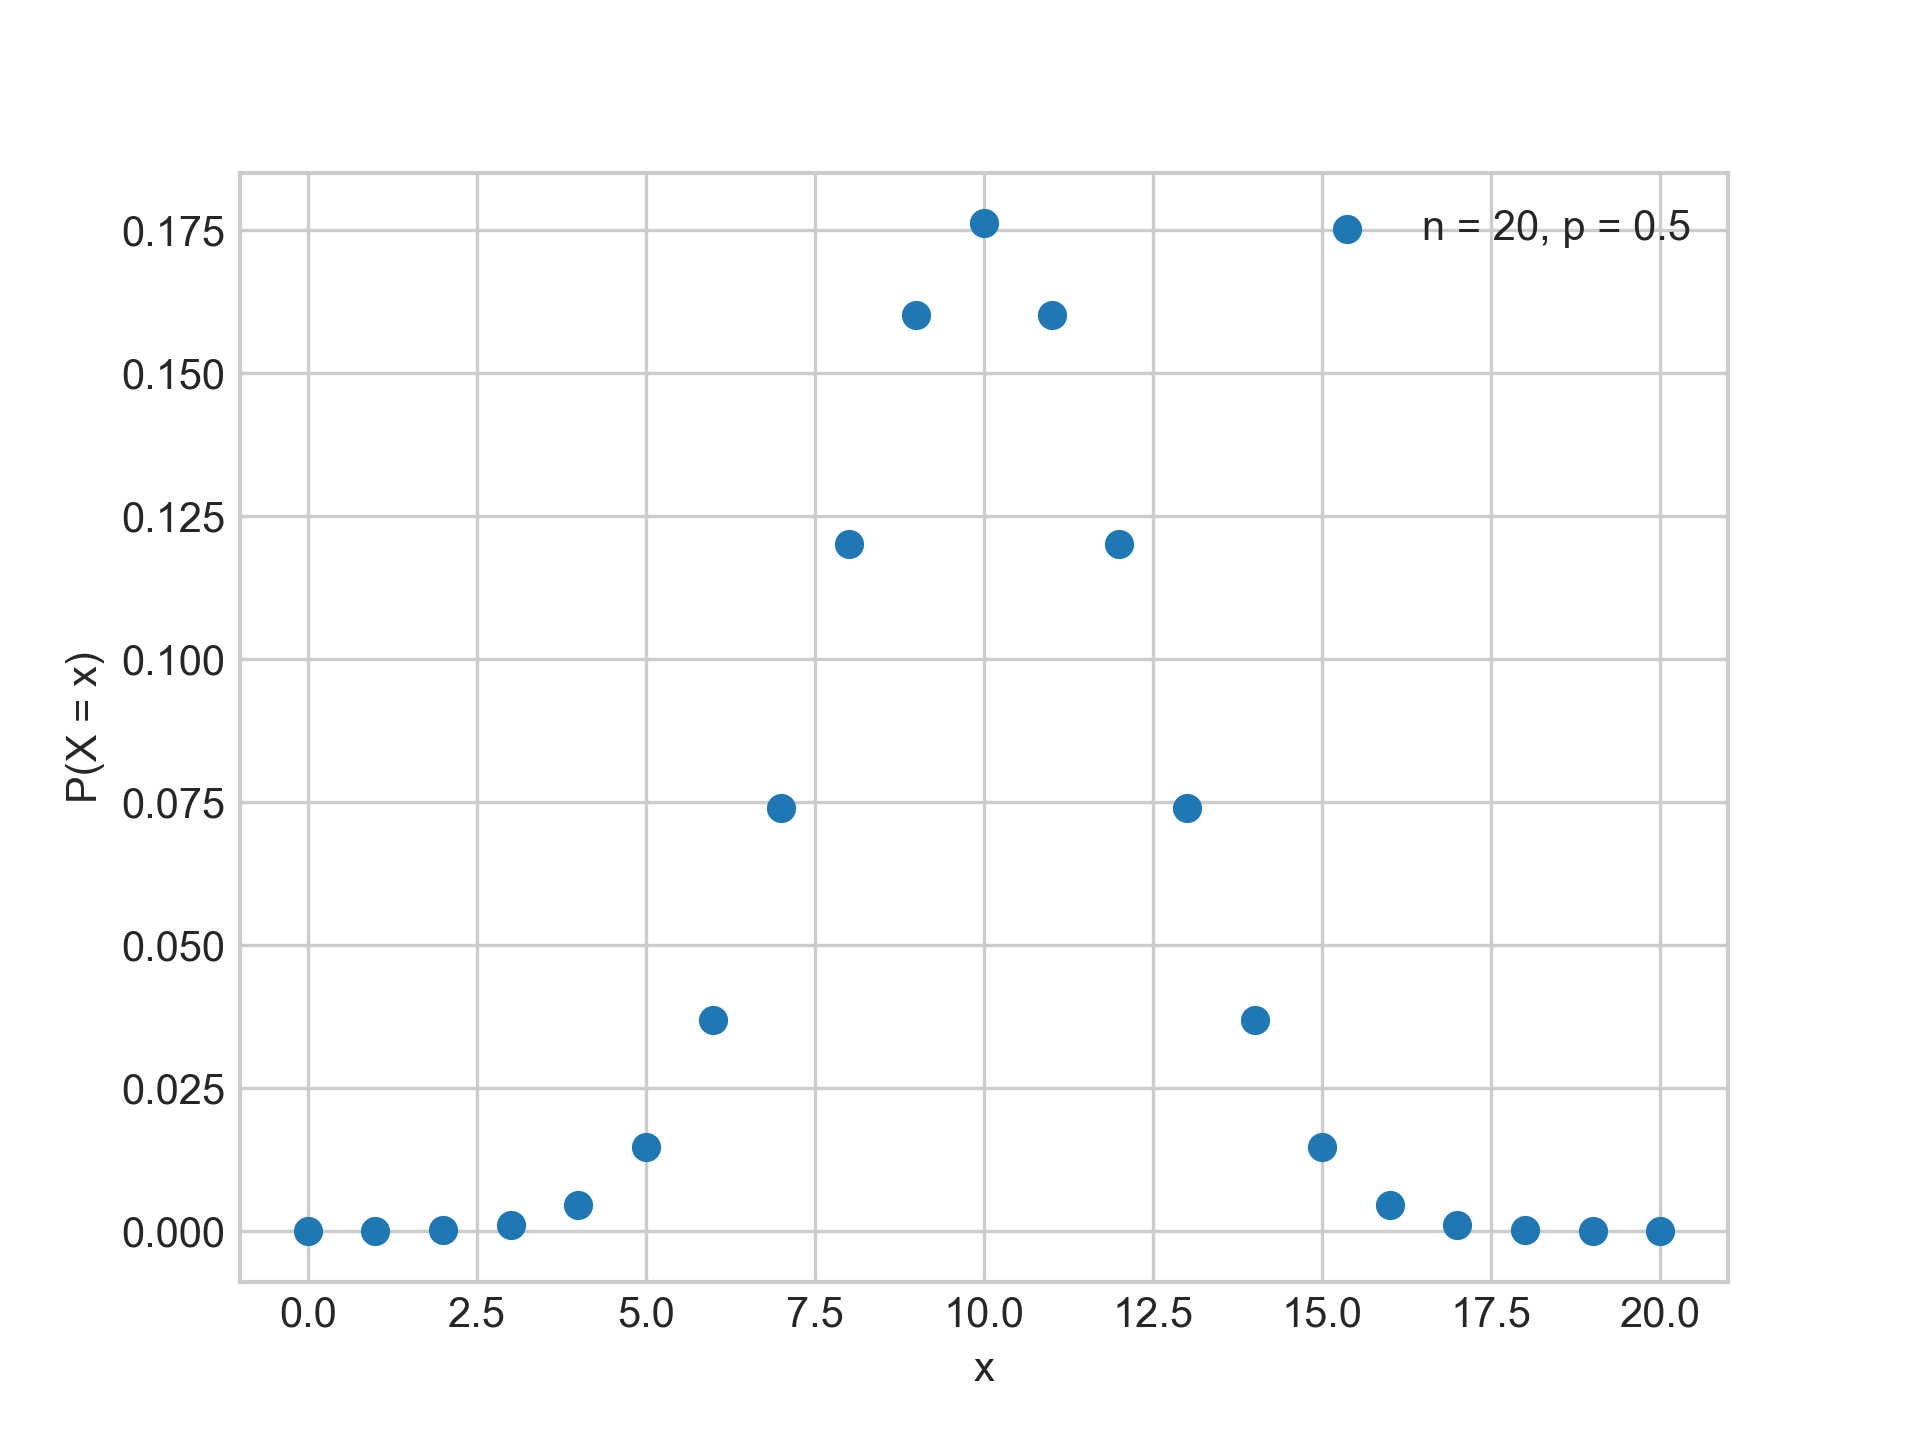
\includegraphics[width=0.4\textwidth]{binomial_pdf.png}
    \captionof{figure}{Probability distribution function of a binomial random variable with p = 0.2 and n = 20.}
    \label{fig:binomial_pdf}
    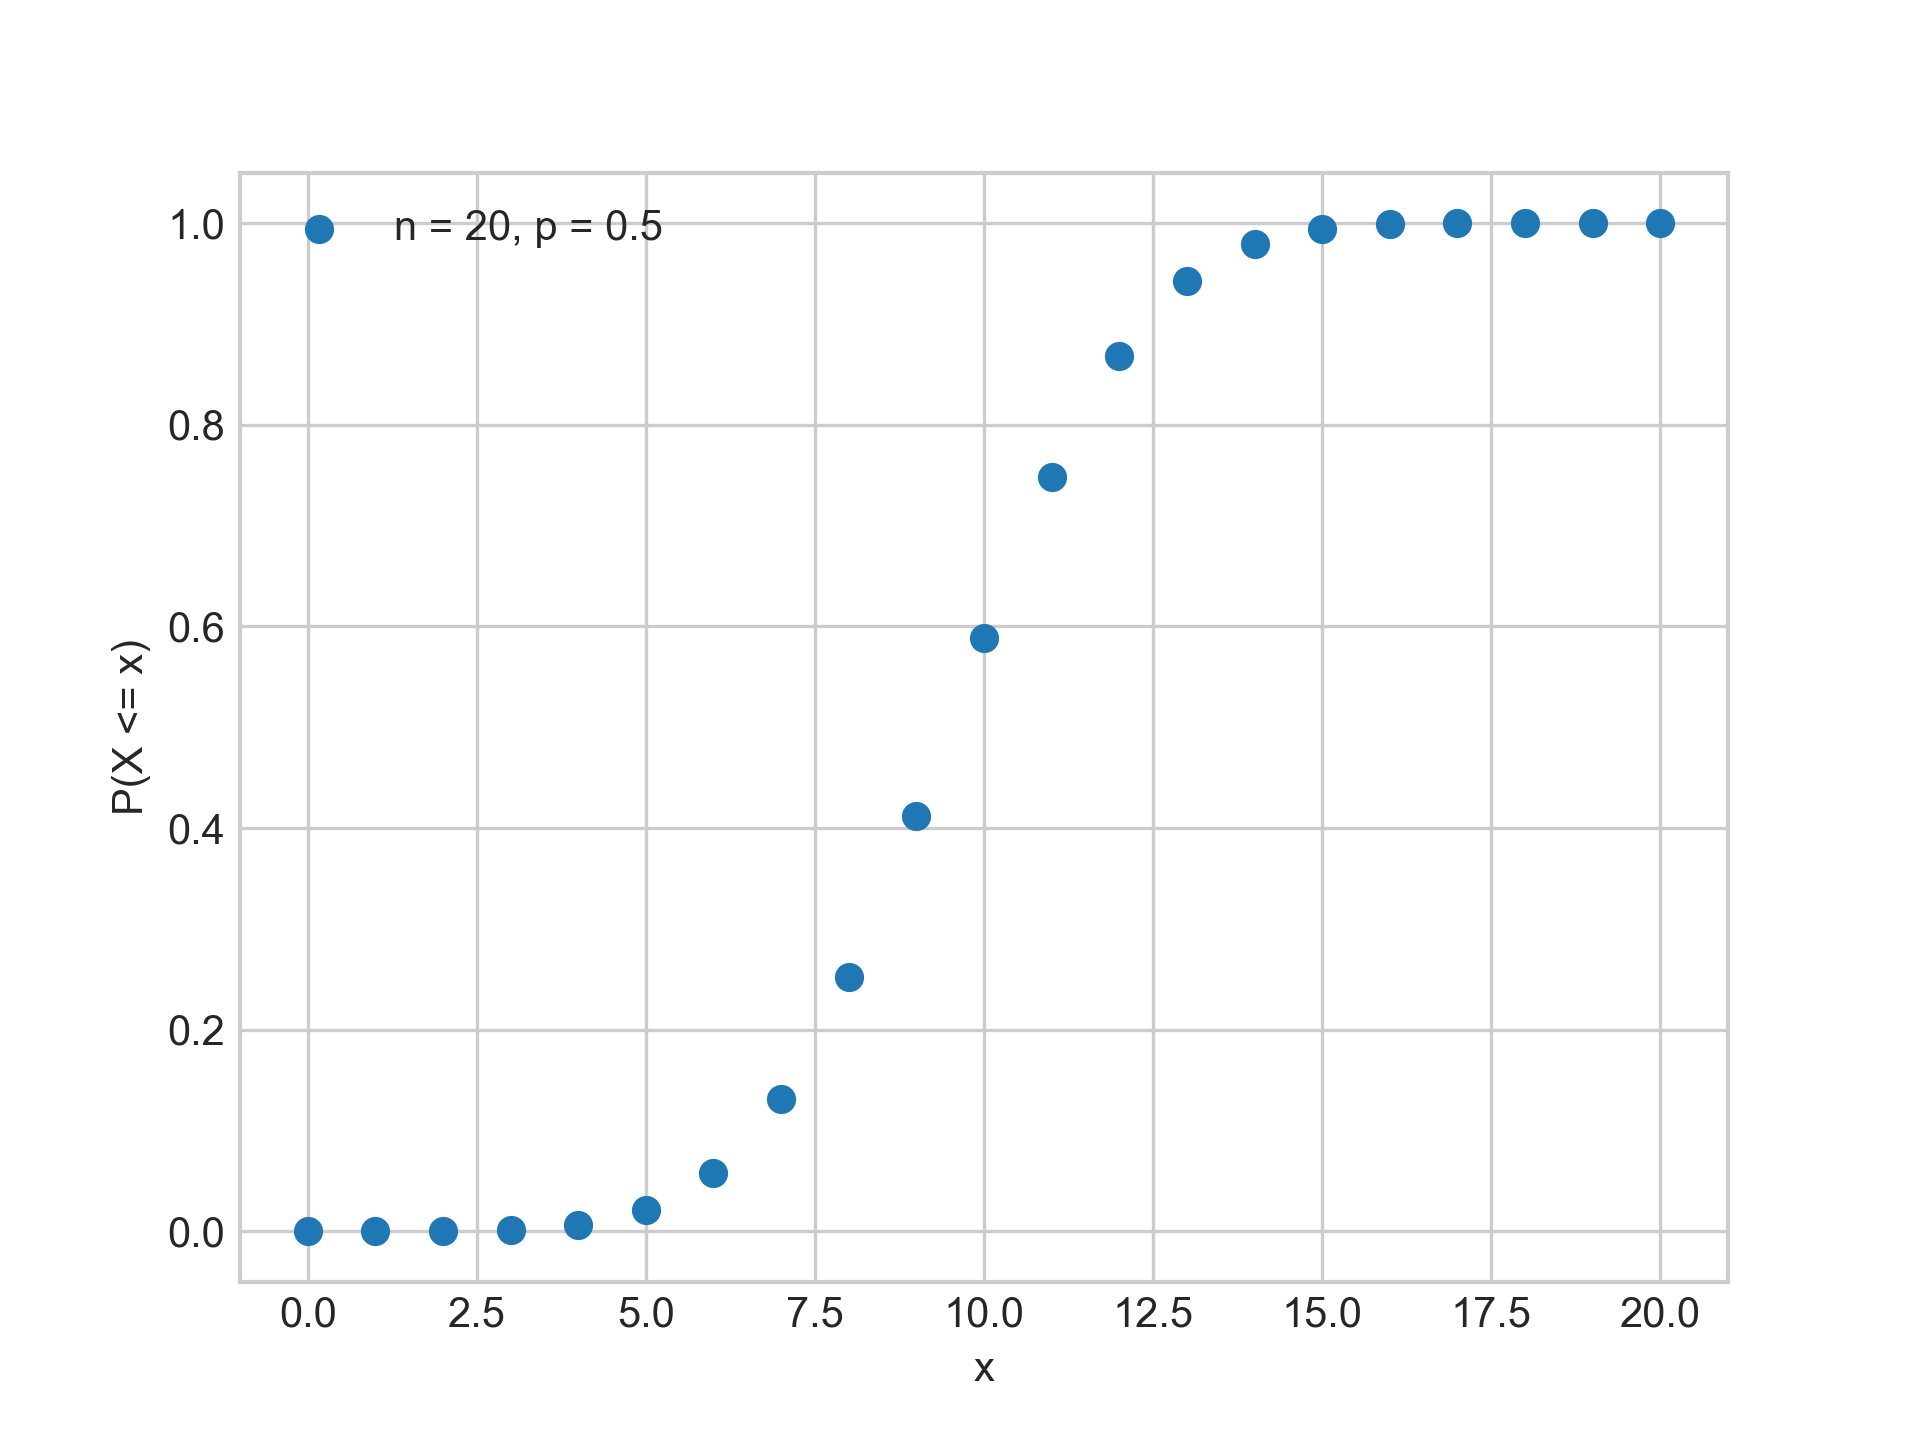
\includegraphics[width=0.4\textwidth]{binomial_cdf.png}
    \captionof{figure}{Cumulative distribution function.}
\end{center}
}:
\begin{equation}
    P(X=k) = \binom{n}{k} p^k q^{n-k}
\end{equation}

\noindent\textbf{What is the link between the binomial and the Bernoulli distribution?}\\
Defining $Y_i$ as the $i^{th}$ Bernoulli random variable, we can say that the sum of $n$ independent Bernoulli random variables is a binomial random variable.
\begin{equation}
    X = \sum_{i=1}^{n} Y_i \sim \text{Bin}(n, p)
\end{equation}

\Example{Adam and Barbara are playing table tennis. In a single game, Barbara wins with probability of $0.6$. If they play a series of $7$ games, what is the probability that Barbara wins exactly $5$ games? Assume that the outcome of each game is independent.}

We can model the number of games Barbara wins as a binomial random variable $X \sim \text{Bin}(7, 0.6)$. The probability of Barbara winning exactly $5$ games is given by:
\[
P(X=5) = \binom{7}{5} 0.6^5 0.4^2
\]

\Example{In the previous setting, what is the probability that Barbara wins at least $5$ games?}

The probability of Barbara winning at least $5$ games is given by:
\[
P(X \geq 5) = P(X=5) + P(X=6) + P(X=7)
\]

\Example{In the previous setting, what is the probability of Barbara winning the last 2 games, given that Barbara won 4 and lost 3 games?}

We need to find the probability that the last two games were wins given that Barbara has 4 wins and 3 losses in total.

The possible scenarios are:
\begin{itemize}
    \item 2 wins, 3 losses in the first 5 games, then 2 wins in the last 2 games.
    \item 3 wins, 2 losses in the first 5 games, then 1 win and 1 loss in the last 2 games.
    \item 4 wins, 1 loss in the first 5 games, then 0 wins in the last 2 games.
\end{itemize}

The only favorable scenario is the first one.

Number of favorable outcomes (2 wins in the last three games): 
$\binom{5}{2} = 10$

Number of possible outcomes: $\binom{7}{4} = 35$

Therefore, the probability is:
\[
P(\text{2 wins in the last 2 games} \mid \text{4 wins and 3 losses}) = \frac{10}{35}
\]

\section{Geometric Distribution}
If $X$ is the number of trials needed to get the first success in a sequence of Bernoulli trials.
\[
P(X=k)
\]

1. For the first success to occur on the \( k \)-th trial, the first \( k-1 \) trials must all result in failures. The probability of failure on each trial is \( 1-p \). Therefore, the probability that the first \( k-1 \) trials all fail is \( (1-p)^{k-1} \).

2. The \( k \)-th trial must be a success. The probability of a success on this trial is \( p \).

Hence, the probability that the first success occurs on the \( k \)-th trial is given by:
\[
P(X = k) = (1-p)^{k-1}p
\]

\Definition{
The geometric distribution is a probability distribution that models the number of Bernoulli trials needed to get the first success.\\
The geometric distribution is characterized by a single parameter:
\begin{itemize}
    \item $p$ - the probability of success in each trial.
\end{itemize}
}{Geometric Distribution}

\[
E[X] = \sum_{k=1}^{+\infty} k(q)^{k-1}p = \frac{1}{p} \qquad Var[X] = \frac{q}{p^2}
\]


\section{Negative Binomial}
If we fix the number of successes desired, and we model the number of trials needed to get the desired number of successes, we get the negative binomial distribution.

\Definition{
The negative binomial distribution is a probability distribution that models the number of Bernoulli trials needed to get a fixed number of successes.\\
The negative binomial distribution is characterized by two parameters:
\begin{itemize}
    \item $n$ - the number of successes desired.
    \item $p$ - the probability of success in each trial.
\end{itemize}
$ X \sim \text{NegBin}(r, p) $
}{Negative Binomial Distribution}

We have $n$ successes in $k$ trials, the number of failures is therefore $k-n$.
Since the last trial must be a success, the number of possible arrangements of outcomes is $\binom{k-1}{n-1}$.
We can then write the probability as:
\[
    P(X=k) = \binom{k-1}{n-1} p^n q^{k-n}
\]

\section{Hypergeometric Distribution}

\Definition{
The hypergeometric distribution is a probability distribution that models the number of successes in a sample of size $n$ drawn without replacement from a finite population of size $N$ that contains $K$ successes.
It is characterized by three parameters:
\begin{itemize}
    \item $N$ - the population size.
    \item $K$ - the number of successes in the population.
    \item $n$ - the sample size.
\end{itemize}
}{Hypergeometric Distribution}

\[
X \sim \text{Hypergeom}(N, K, n)
\]

The probability distribution function of $X$ is given by:
\[
P(X=k) = \frac{\binom{K}{k} \binom{N-K}{n-k}}{\binom{N}{n}}
\]

Its expected value is:
\[
E[X] = n \frac{K}{N}
\]


\setchapterabstract{This chapter is dedicated to continuous probability distributions. We start by introducing the Poisson distribution, which models the number of events occurring in a fixed interval of time or space. We then move on to the exponential distribution, which models the time until the first event occurs in a Poisson process. We also introduce the gamma distribution, which models the sum of $n$ exponential random variables. Finally, we introduce the uniform distribution, which models the probability of all outcomes in an interval being equally likely.}
\chapter{Continuous Probability Distributions}
\vspace{-1.5cm}

{\chaptoc\noindent\begin{minipage}[inner sep=0,outer sep=0]{0.9\linewidth}\section{Poission Distribution}\end{minipage}}

This is the continuous time equivalent of a bernoulli random variable. It is used to model the number of events occurring in an interval of time or space.

An example is the number of phone calls received by a person. At any given time, the number of calls received is either zero or one, modeled by a Poisson distribution.

Fixing the time interval $[0, T]$, $X =\text{ number of events in }[0, T]$ is a Poisson random variable\sn{
    \begin{center}
        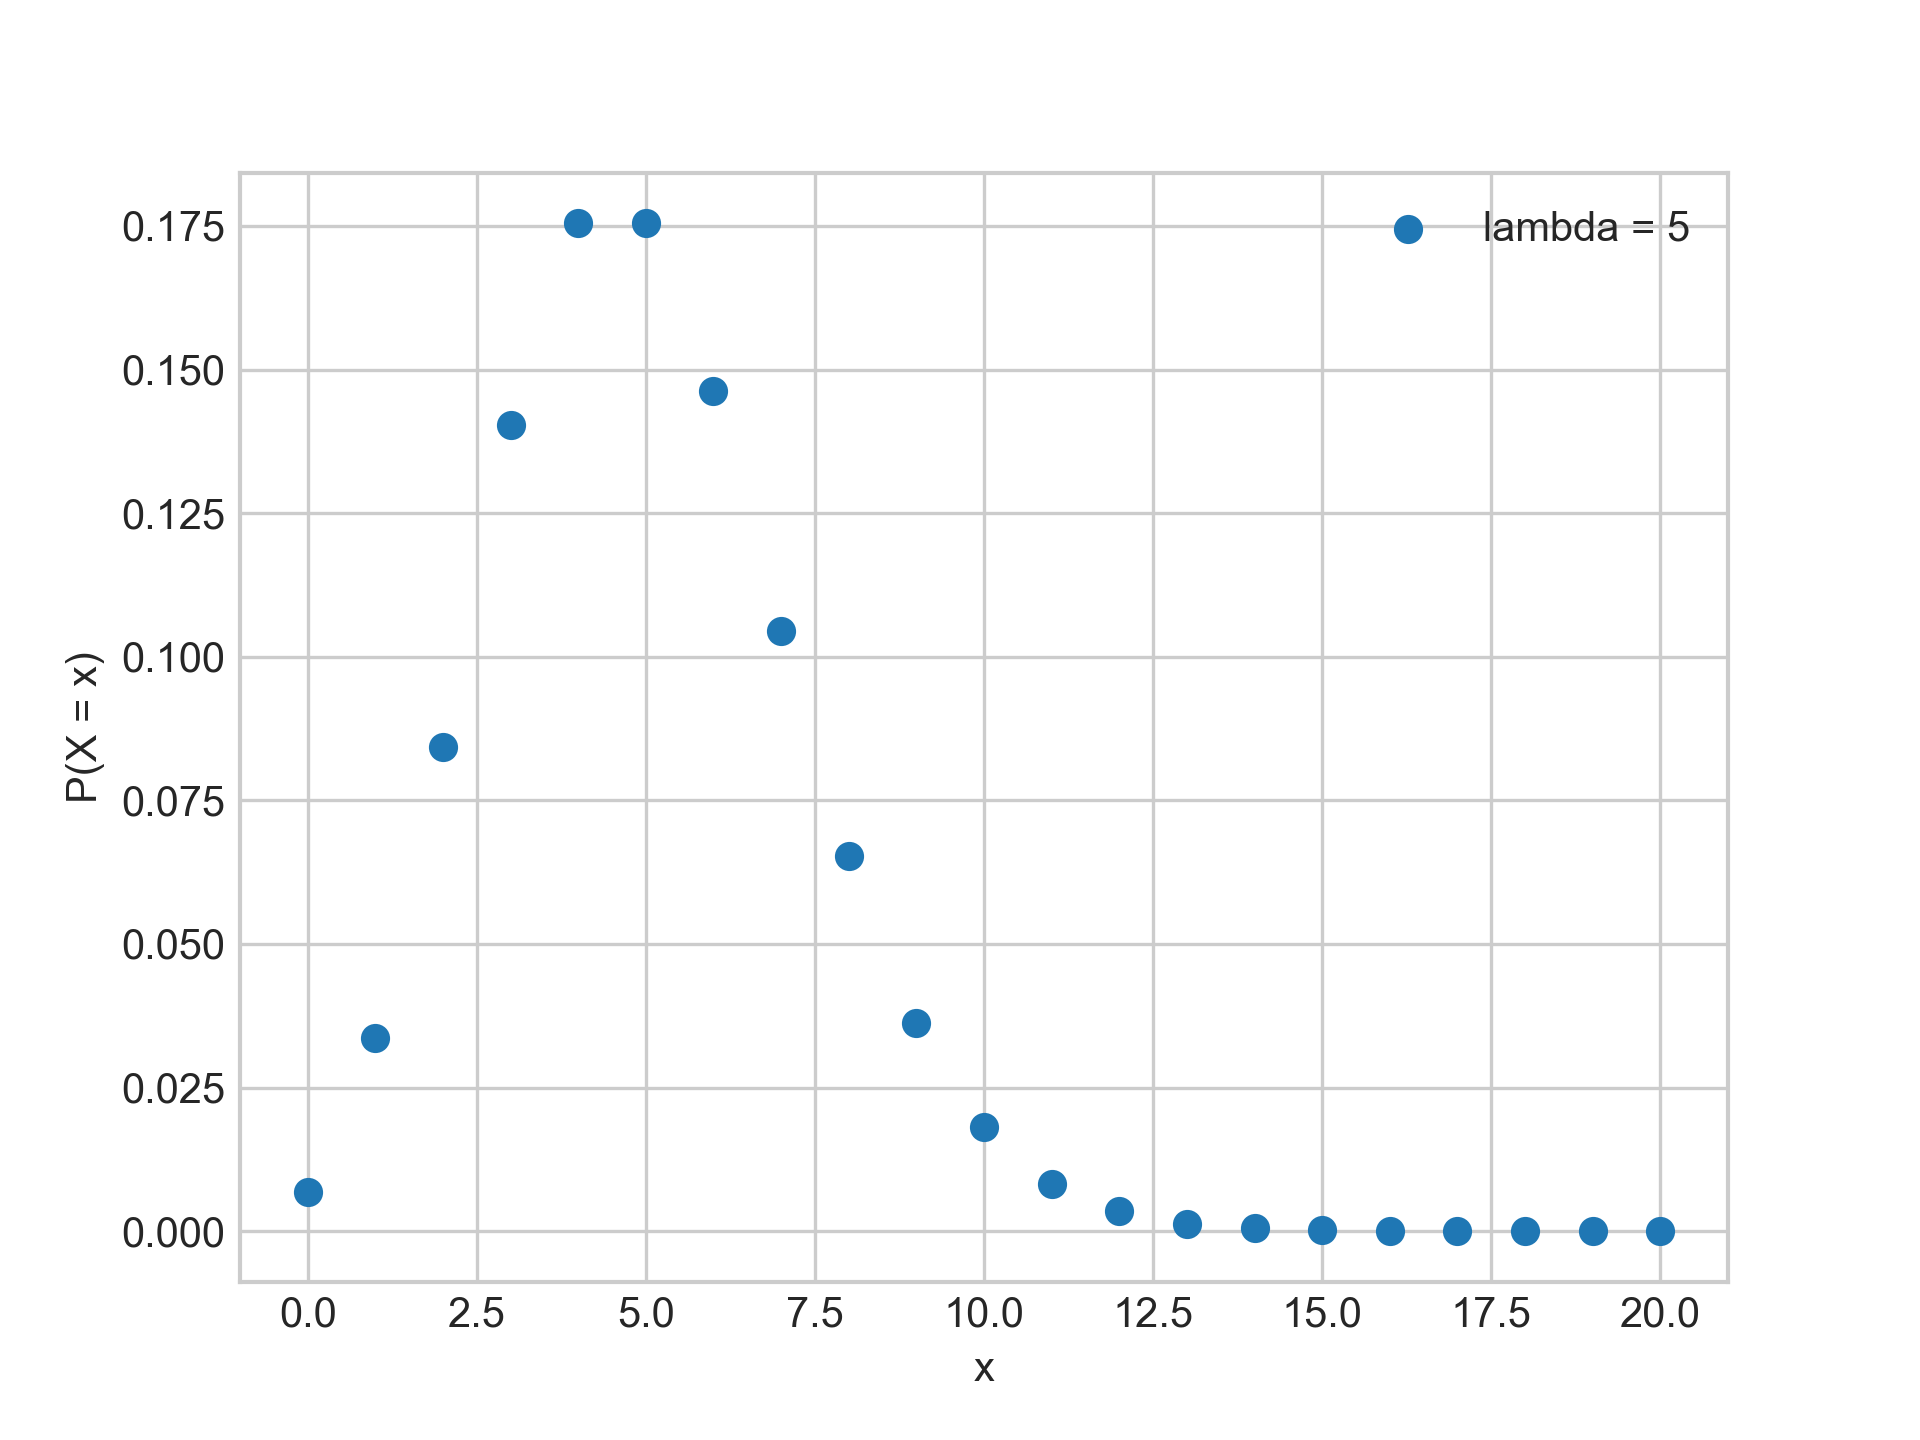
\includegraphics[width=0.4\textwidth]{poisson_pdf.png}
        \captionof{figure}{Probability distribution function of a Poisson random variable with $\lambda = 5$.}
        \label{fig:poisson_pdf}
        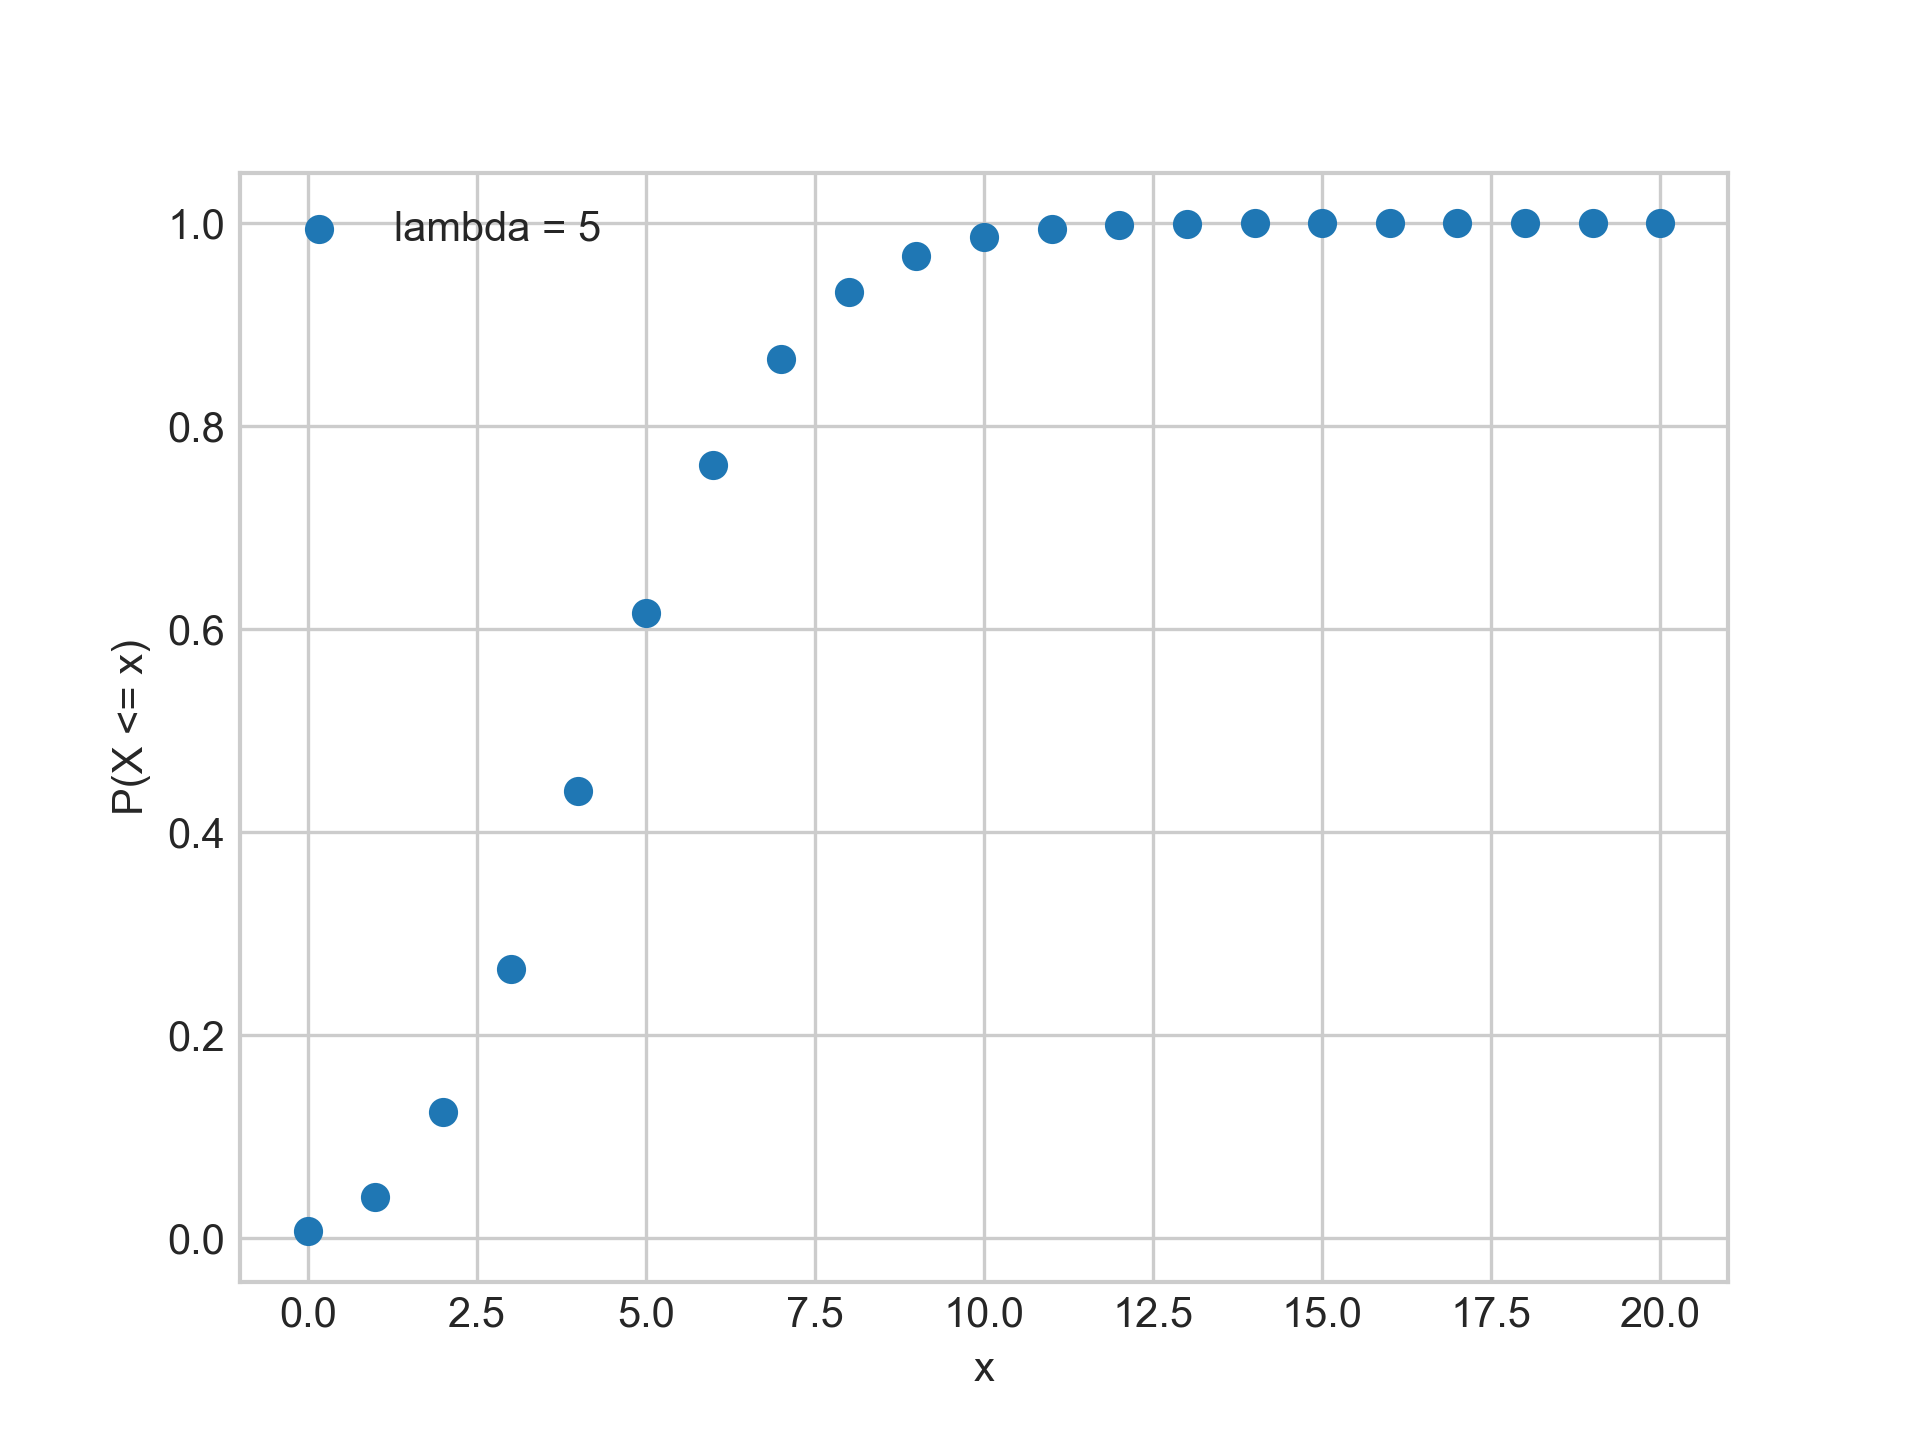
\includegraphics[width=0.4\textwidth]{poisson_cdf.png}
        \captionof{figure}{Cumulative distribution function.}
    \end{center}
}.

\Definition{
The Poisson distribution is a probability distribution that models the number of events occurring in a fixed interval of time or space.\\
The Poisson distribution is characterized by a single parameter:
\begin{itemize}
    \item $\lambda$ - the average rate of events occurring in the interval
    \[\lambda = \frac{\text{number of arrivals}}{\text{time interval}}\]
\end{itemize}
}{Poisson Distribution}

The probability of having 1 arrival in a time interval is given by:
\[
P(X=1) \approx \lambda \Delta t 
\]
\[
P(X=1) = \lambda \Delta t + o(\Delta t)
\]

The probability distribution function of a Poisson random variable is given by:
\[
P(X=k) = \frac{e^{-\lambda T} (\lambda T)^k}{k!}
\]

\section{Exponential Distribution}

If $X$ is the waiting time until the first event occurs in a Poisson process, then $X$ is an exponential random variable

\Definition{
The exponential distribution is a probability distribution that models the time until the first event occurs in a Poisson process.\\
The exponential distribution is characterized by a single parameter:
\begin{itemize}
    \item $\lambda$ - the rate of events occurring in the Poisson process.
\end{itemize}
}{Exponential Distribution}

The probability distribution function of an exponential random variable is given by \sn{
    \begin{center}
        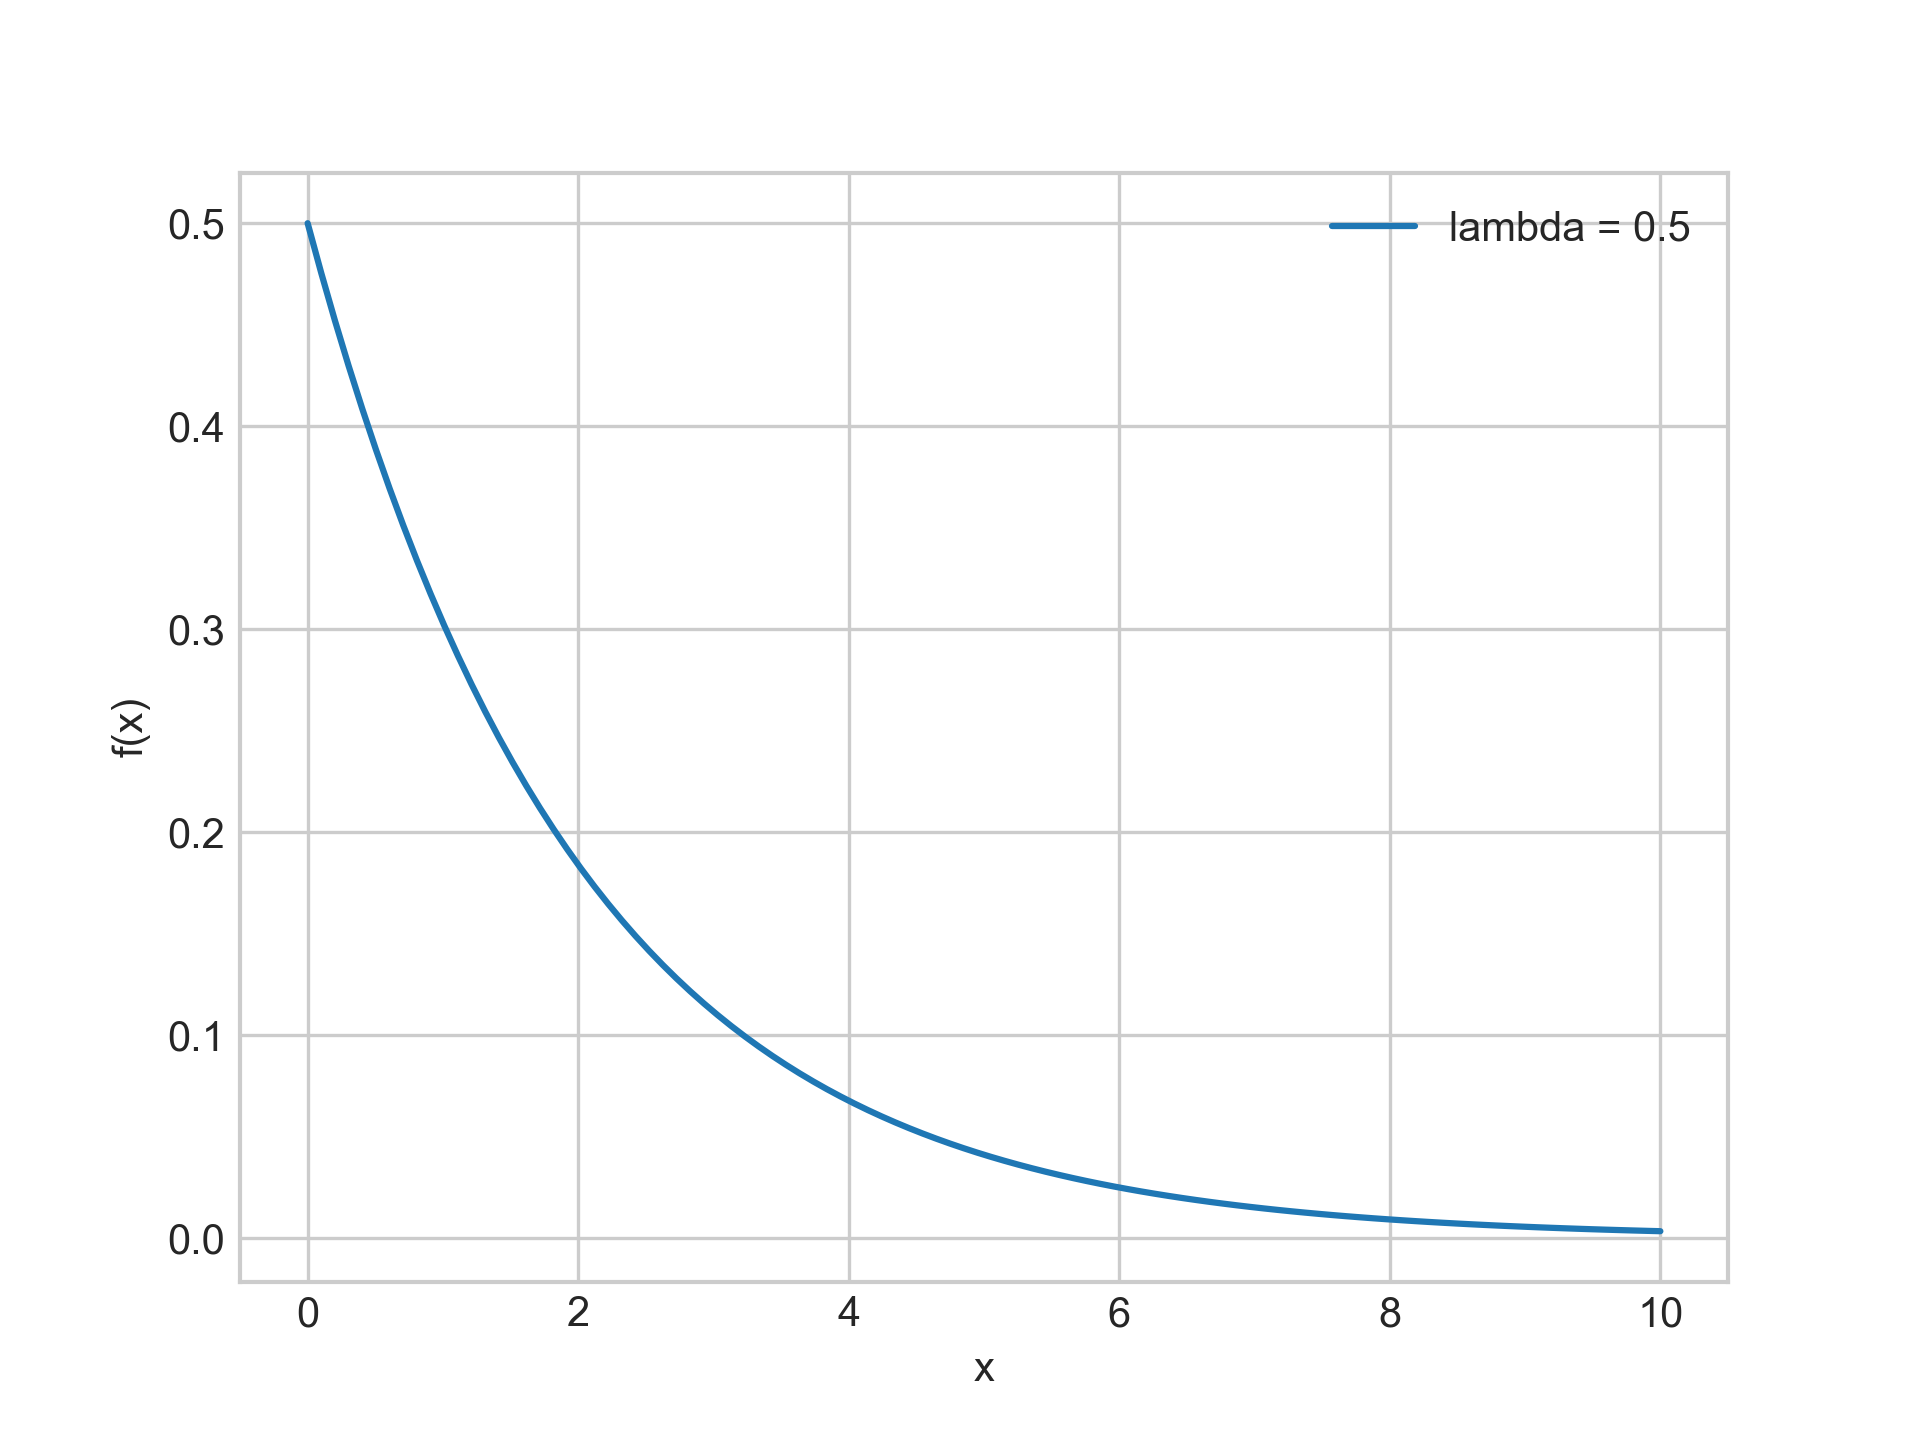
\includegraphics[width=0.4\textwidth]{exponential_pdf.png}
        \captionof{figure}{Probability distribution function of an exponential random variable with $\lambda = 0.5$.}
        \label{fig:exponential_pdf}
        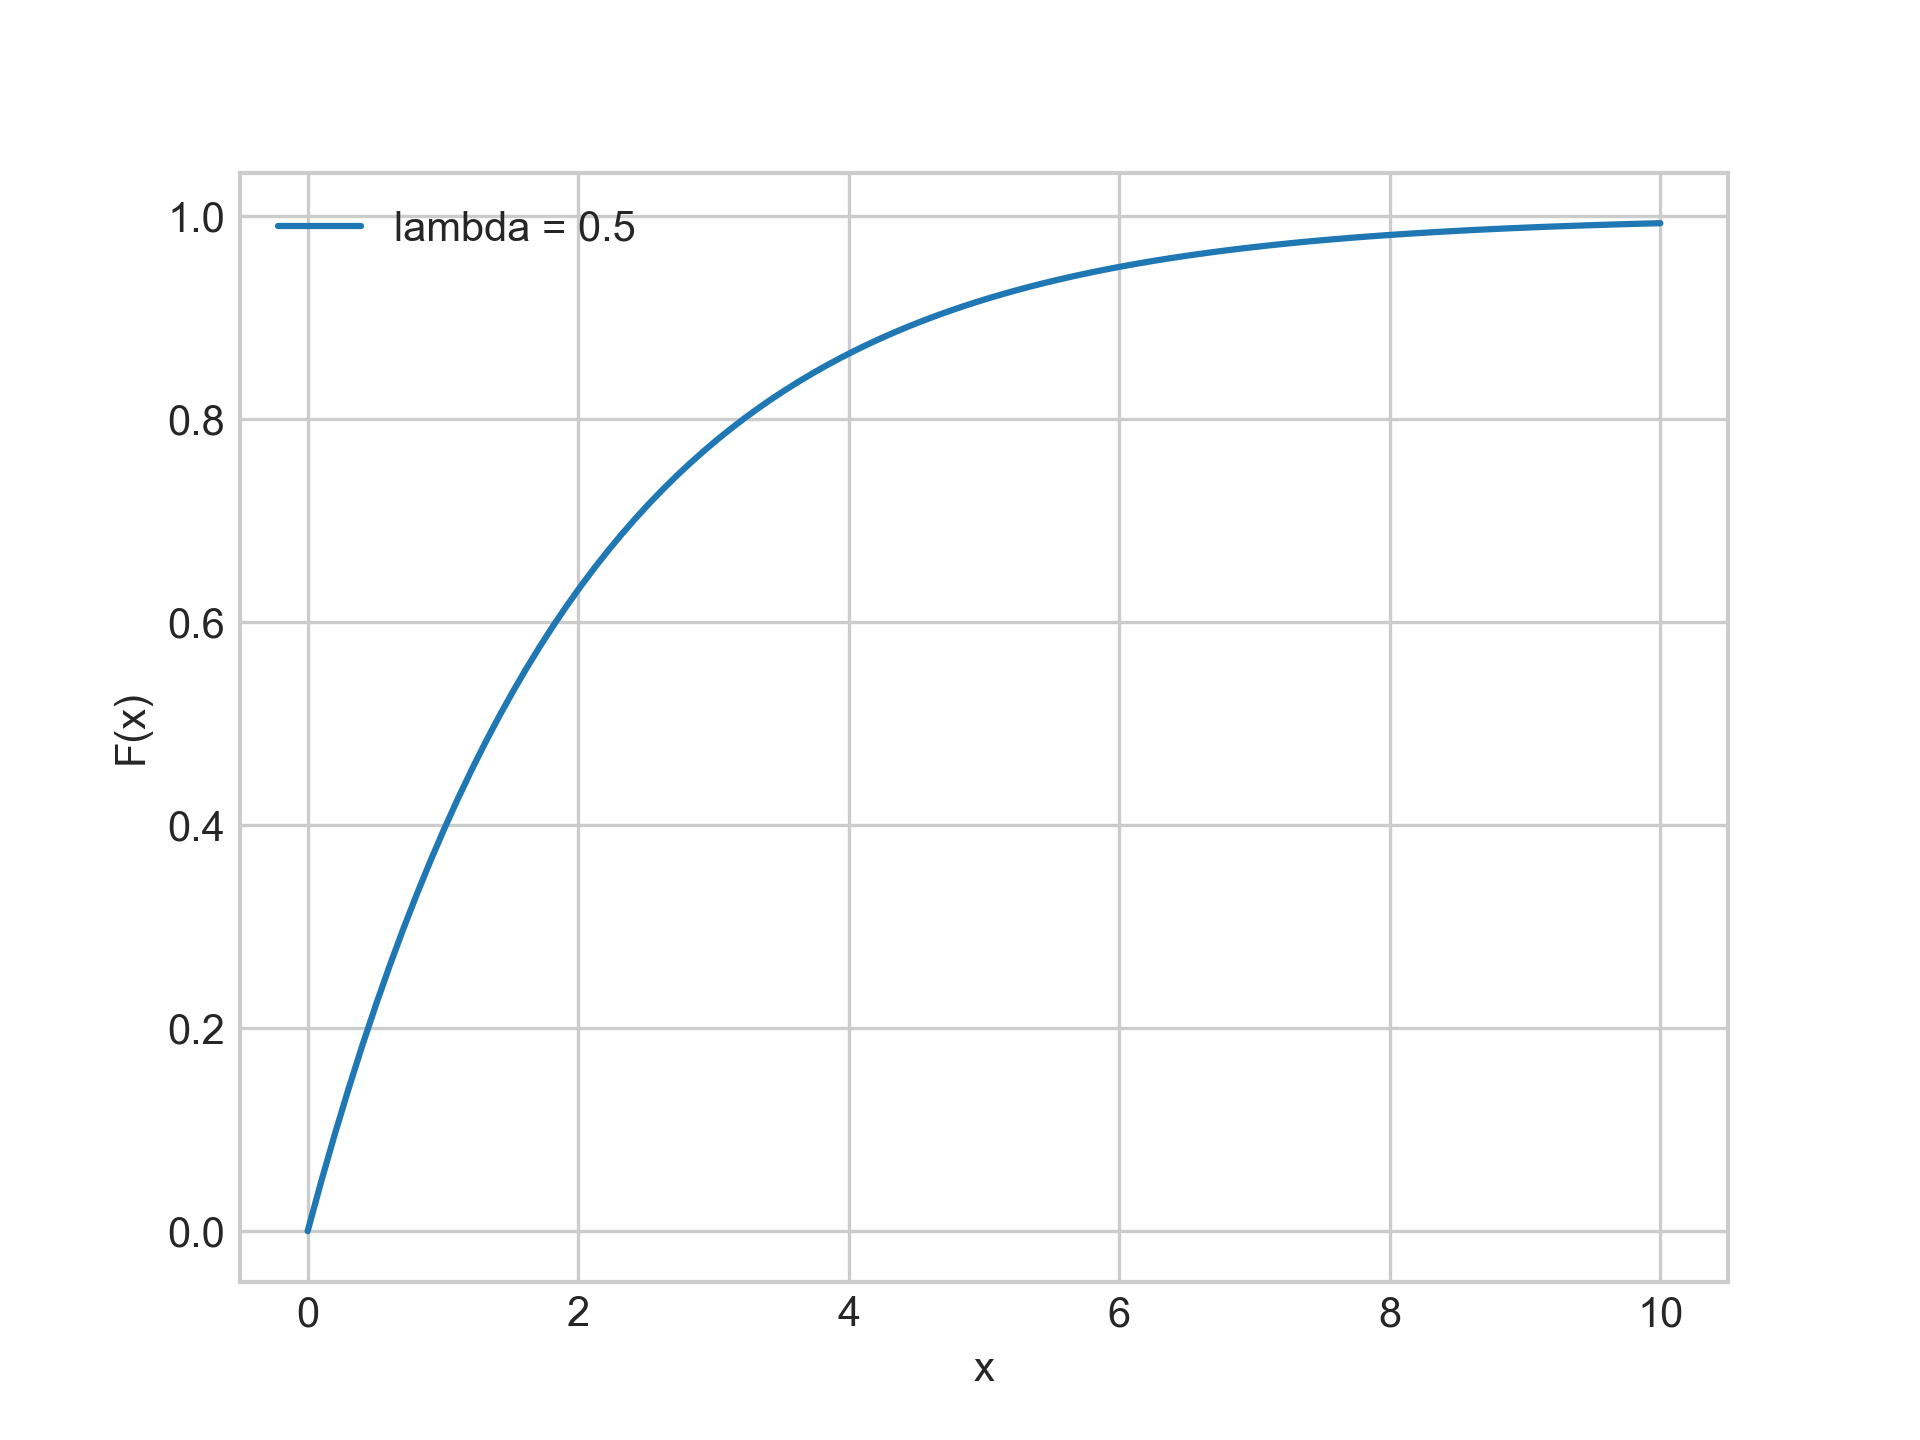
\includegraphics[width=0.4\textwidth]{exponential_cdf.png}
        \captionof{figure}{Cumulative distribution function.}
    \end{center}
}:
\[
f(x) = 
\begin{cases}
    \lambda e^{-\lambda x} & x \geq 0 \\
    0 & x < 0
\end{cases}
\]

The expected value and variance of an exponential random variable are given by:
\[
E[T] = \int_{0}^{+\infty} x f(x) dx = \frac{1}{\lambda} \qquad Var[T] = \frac{1}{\lambda^2}
\]

The exponential distribution is memoryless, meaning that the probability of an event occurring in the next interval (waiting time) is independent of the time that has already passed.


\section{Gamma Distribution}
\Definition{
The gamma function is defined as:\\
\[
\Gamma(z) = \int_{0}^{+\infty} x^{z-1} e^{-x} dx
\]
It is defined as long as the exponent $z$ is positive.
}{Gamma Function}


Properties of the gamma function:
\begin{itemize}
    \item $\Gamma(z+1) = z\Gamma(z)$
    \item $\Gamma(1) = 1$
    \item $\Gamma(n+1) = n!$
\end{itemize}

The most important property of the gamma function is its recursive definition\sn{
    Integration by part:
    \[
    \int u dv = uv - \int v du
    \]
}:
\Proposition{
\[ \Gamma(z+1) = z\Gamma(z) \]
}{
    \begin{equation}
        \begin{aligned}
            \Gamma(z+1) & = \int_{0}^{+\infty} x^z e^{-x} dx \\
            & = \left[-x^z e^{-x}\right]_{0}^{+\infty} + z\int_{0}^{+\infty} x^{z-1} e^{-x} dx = z\Gamma(z)
        \end{aligned}
        \end{equation}
}

From this property, we can see that the gamma function is a generalization of the factorial function. For any positive integer $n$, we have $\Gamma(n+1) = n!$.

Starting from the gamma function, we can define the gamma distribution\sn{
    \begin{center}
        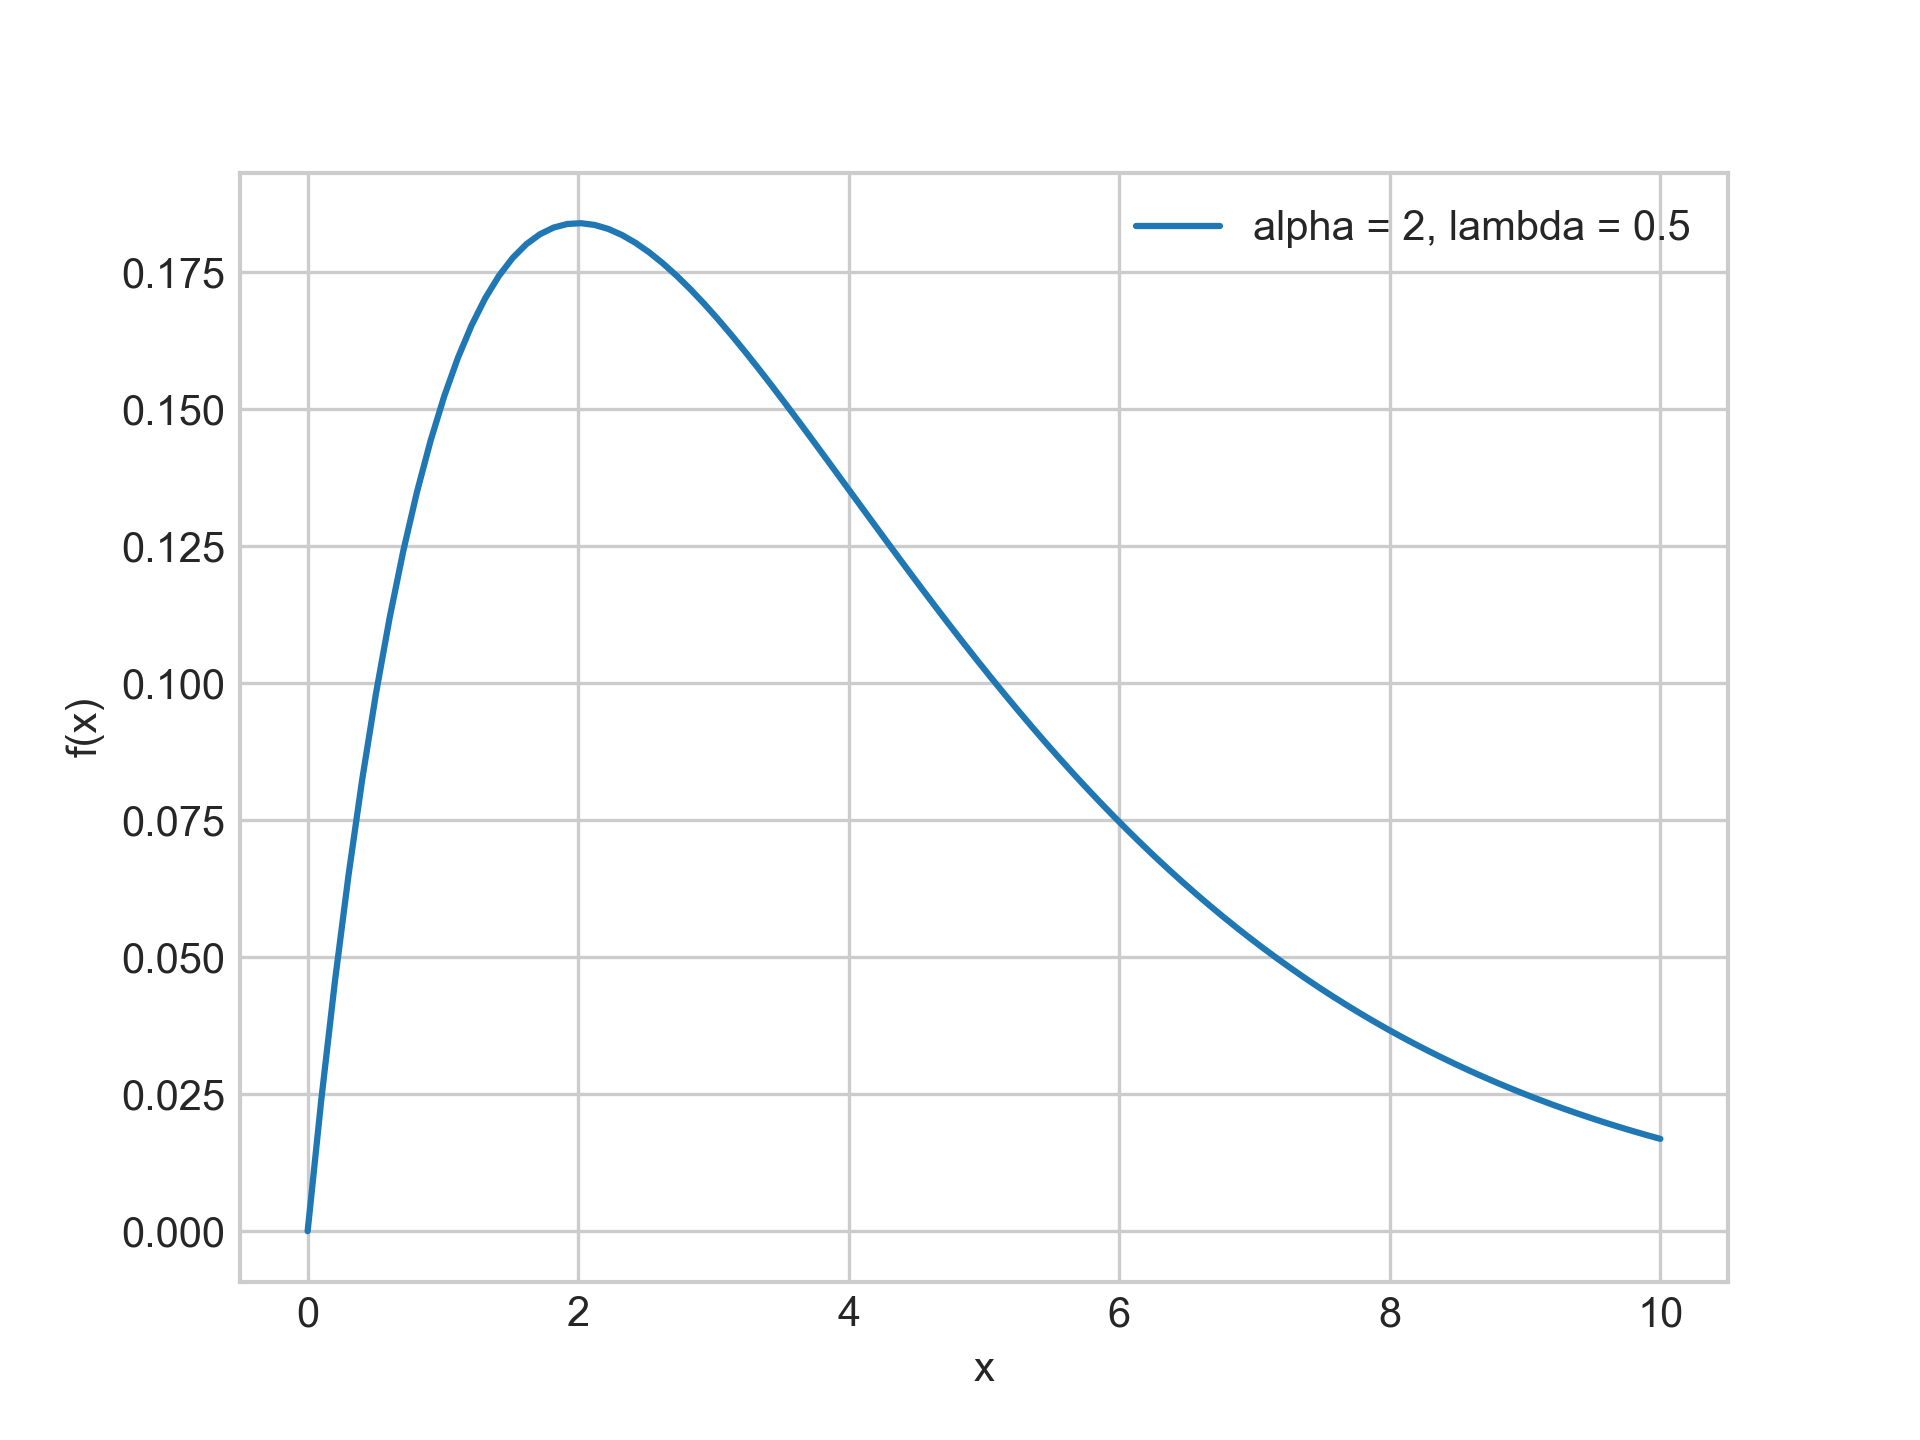
\includegraphics[width=0.4\textwidth]{gamma_pdf.png}
        \captionof{figure}{Probability distribution function of a gamma random variable with $\alpha = 2$ and $\lambda = 0.5$.}
        \label{fig:gamma_pdf}
        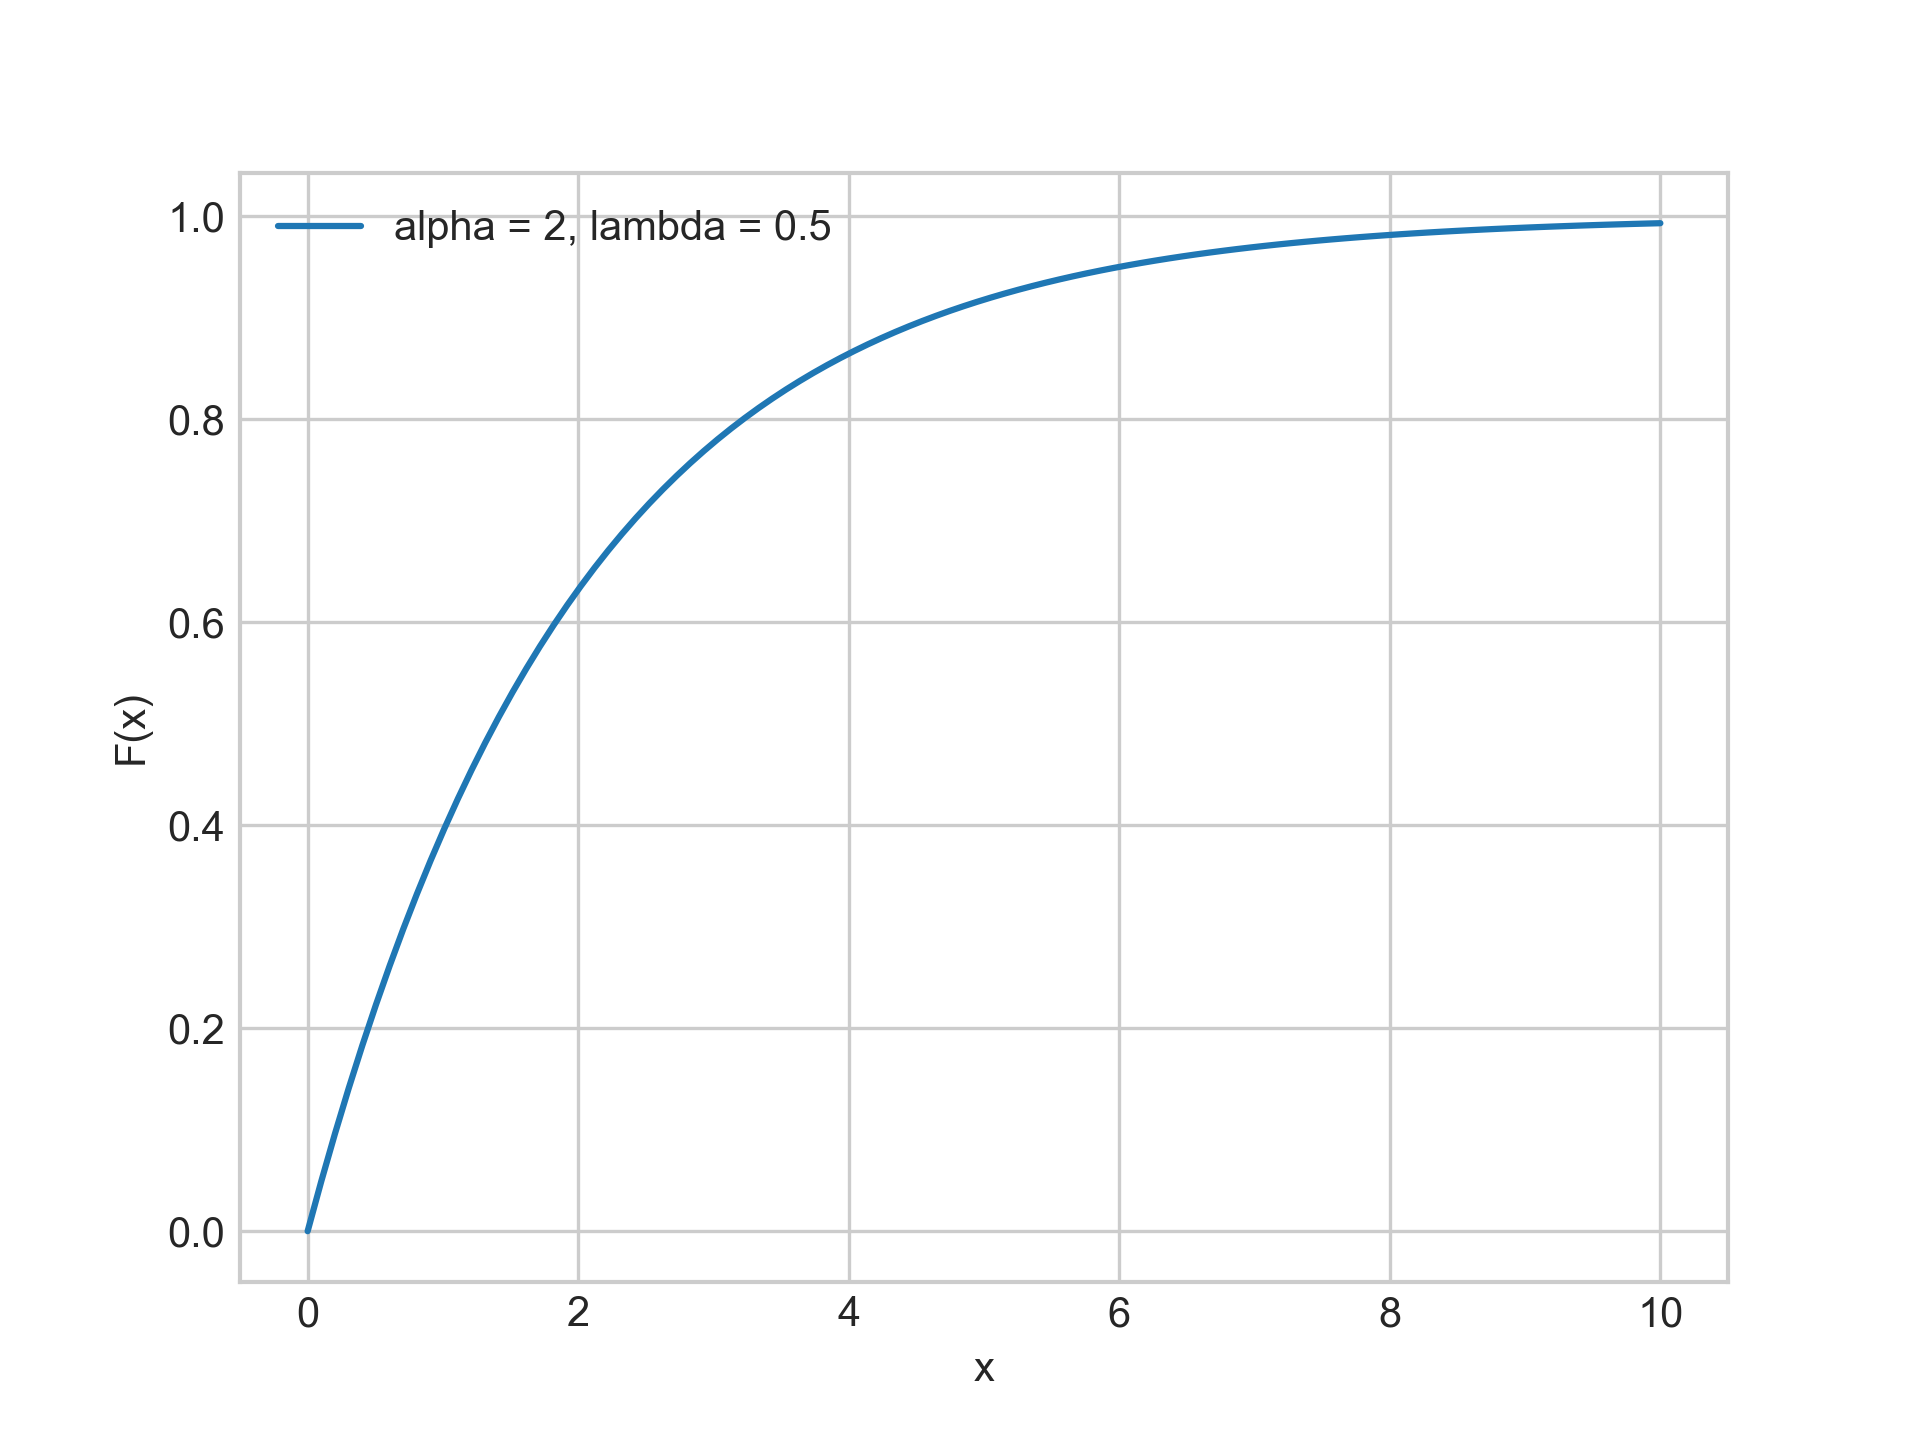
\includegraphics[width=0.4\textwidth]{gamma_cdf.png}
        \captionof{figure}{Cumulative distribution function.}
    \end{center}
}.

\Definition{
The gamma distribution is a probability distribution that models the sum of $n$ exponential random variables.\\
The gamma distribution is characterized by two parameters:
\begin{itemize}
    \item $n$ - the number of exponential random variables.
    \item $\lambda$ - the rate of events occurring in the Poisson process.
\end{itemize}
\[ X \sim \text{Ga}(\alpha, \lambda) \]
\[
f(x) = 
\begin{cases}
    \frac{\lambda^{\alpha}}{\Gamma(\alpha)} x^{\alpha-1} e^{-\lambda x} & x \geq 0 \\
    0 & x < 0
\end{cases}
\]
}{Gamma Distribution}

\Proposition{
The expected value of $X\sim \text{Ga}(\alpha, \lambda)$ is given by:
\[
E[X] = \frac{\alpha}{\lambda}
\]
}{
    \begin{equation}
        \begin{aligned}
            E[X] &= \int_{0}^{+\infty} x f(x) dx = \int_{0}^{+\infty} x \frac{\lambda^{\alpha}}{\Gamma(\alpha)} x^{\alpha-1} e^{-\lambda x} dx \\
                &=  \int_{0}^{+\infty} \frac{\lambda^{\alpha}}{\Gamma(\alpha)} x^{\alpha}e^{-\lambda x}
        \end{aligned}
    \end{equation}
    We can see that this is similar to the integral of the gamma function with $\alpha = \alpha +1$, to make it equal, we need to multiply by $\frac{\lambda}{\lambda}$.
    \begin{equation}
        \begin{aligned}
            E[X] &= \frac{1}{\lambda} \overbrace{\frac{\Gamma(\alpha+1)}{\Gamma(\alpha)}}^{=\alpha \Gamma(\alpha)} \underbrace{
            \int_{0}^{+\infty} \frac{\lambda^{\alpha+1}}{\Gamma(\alpha+1)} x^{\alpha}e^{-\lambda x} dx}_{= 1} \\
            &= \frac{\alpha}{\lambda}
        \end{aligned}
    \end{equation}
}


\section{Uniform Distribution}

If all outcomes in an interval are equally likely, we have a uniform distribution.
Its probability distribution function is given by:
\[
f(x) = \begin{cases}
    \frac{1}{b-a} & a \leq x \leq b \\
    0 & \text{otherwise}
\end{cases}
\]

The cumulative distribution function is:
\[
F(t) = \begin{cases}
    0 & x < a \\
    \frac{t-a}{b-a} & a \leq x \leq b \\
    1 & x > b
\end{cases}
\]

The expected value and variance of a uniform random variable are given by:
\[
E[X] = \frac{a+b}{2} \qquad Var[X] = \frac{(b-a)^2}{12}
\]

